\section{Aufbau}
\label{sec:Aufbau}

Der verwendete Versuchsaufbau ist in Abbildung \ref{fig:aufbau} dargestellt.
\begin{figure}
\centering
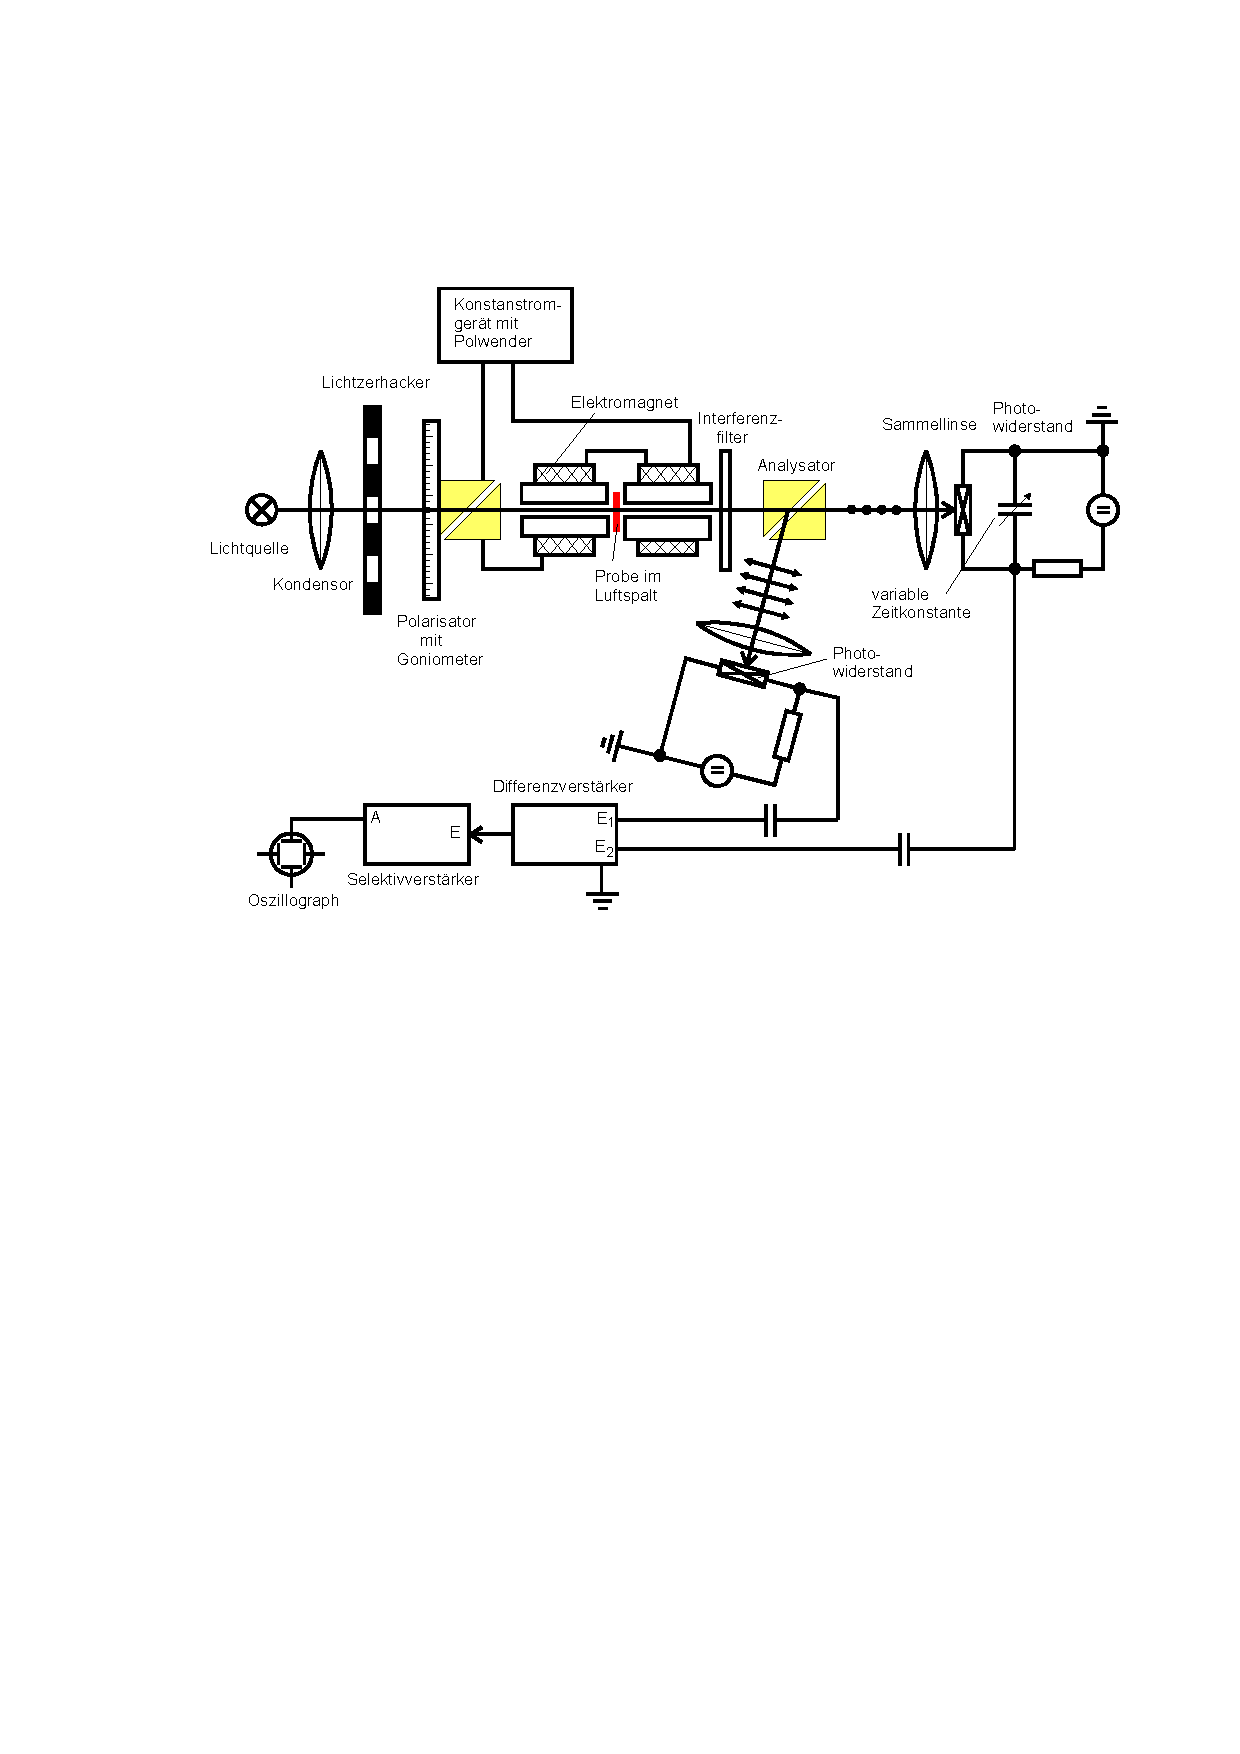
\includegraphics[width=0.7\linewidth]{./content/images/aufbau.pdf}
\caption{Schematische Darstellung des Versuchsaufbaues.}
\label{fig:aufbau}
\end{figure}
Das Experiment verwendet als Lichtquelle eine Halogenlampe, deren Emissionsspektrum
hauptsächlich im Infrarotbereich liegt.
Das emittierte Licht wird von einer Kondensorlinse gesammelt und als paralleler Strahl in den weiteren Versuchsaufbau geleitet (siehe. Abb. \ref{fig:kondensorlinse}).
\begin{figure}
\centering
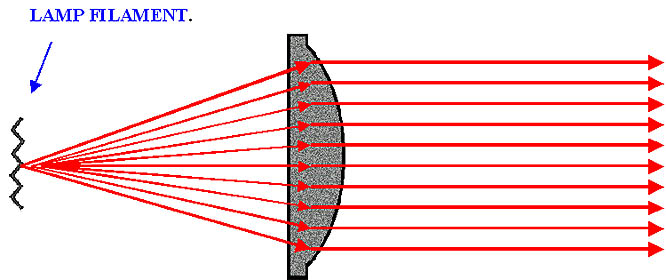
\includegraphics[width=0.45\linewidth]{./content/images/condensor.jpeg}
\caption{Schematische Strahlengang von Licht vor und nach einer Kondensorlinse.}
\label{fig:kondensorlinse}
\end{figure}
Das von der Kondensorlinse gesammelte Licht gelangt über einen Lichtzerhacker in
ein Glan-Thompson-Prisma.
Dieses Prisma besteht aus Kalkspat und erzeugt das für die Messung notwendige linear polarisierte Licht (vgl. Abb. \ref{fig:glan_thompson_prisma}).
\begin{figure}
\centering
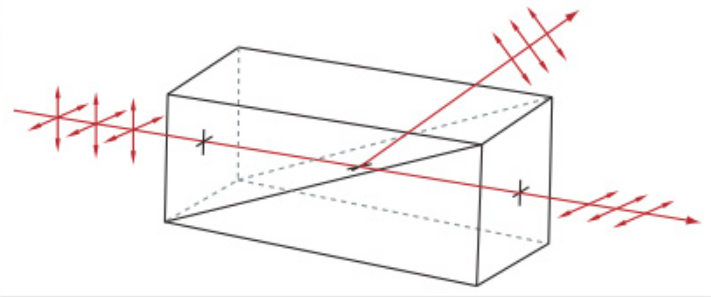
\includegraphics[width=0.5\linewidth]{./content/images/glan_thompson_prisma.png}
\caption{Schematische Darstellung eines Glan-Thompson-Prisma als Strahlenteiler.
Die Polarisationsebenen der beiden austretenden Strahlen stehen orthogonal aufeiannder.}
\label{fig:glan_thompson_prisma}
\end{figure}
Das polarisierte Licht trifft auf die Probe, welche sich in einem durch einen Elektromagneten erzeugten Magnetfeld befindet.
Zu betonen ist, dass der Wellenvektor des Lichtfeldes parallel zum zeitlich konstanten Magnetfeldvektor liegt.
Als Proben werden zwei n-dotierte und ein reiner Galliumarsenid-Kristalle untersucht.
Die beiden n-dotierten Kristalle unterscheiden sich in ihrer Dicke und Dotierungsstärke.
Nach dem Austreten aus der Probe wird das Wellenlängenspektrum des Lichts mit Hilfe
eins Interferenzfilters auf eine Wellenlänge reduziert.
Ein Interferenzfilter besteht aus zwei semitransparenten Schichten die eine transparentes Dielektrikum umgeben (siehe Abb. \ref{fig:interferenzfilter}).
Das eintretende Licht wird durch die reflektierenden
Außenschichten mehrmals reflektiert, was zu Interferenzen führt.
Mit Hilfe dieser Interferenzen ist es möglich, durch Variierung der
Dicke des Filters, nur bestimmte Wellenlängen passieren zu lassen.
\begin{figure}
\centering
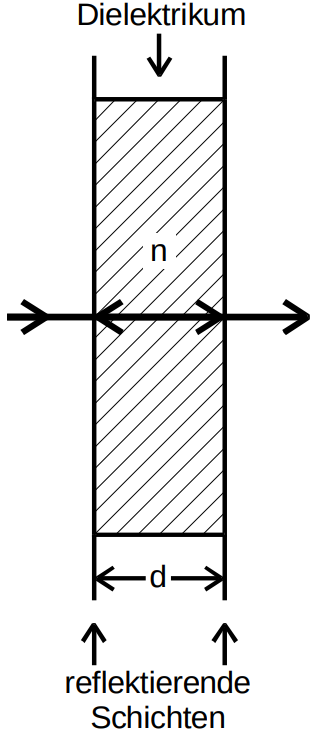
\includegraphics[width=0.15\linewidth]{./content/images/interferenzfilter.png}
\caption{Schmeatischer Aufbau eines Interfernzfilters.}
\label{fig:interferenzfilter}
\end{figure}
Das monochromatische Licht trifft anschließend auf ein zweites Glan-Thompson-Prisma,
das zwei Teilstrahlen unterschiedlicher Polarisation erzeugt.
Die Intensität der beiden ausgehenden Strahlen hängt dabei von der Polarisation des eingehenden Strahls ab.
Die beiden Teilstrahlen werden mit Hilfe von Sammellinsen auf jeweils eine Photodiode fokussiert.
Die Photodioden wandeln die Intensität des auftretenden Lichtes in einen Strom um.
Das Signal der beiden Photodioden wird auf einen Differenzverstärker gegeben, welcher
beide Signale voneinander subtrahiert und die resultierende Differenz verstärkt.
Die dem Balance Schema folgende Messmethode bietet eine besonders hohe Genauigkeit.
Das Signal des Differenzverstärkers wird zu einem Selektivverstärker weitergeleitet.
Mit dem Selektivverstärker soll die Genauigkeit der Messung weiter verbessert werden.
Hierfür wird die Verstärkerfrequenz des Selektivverstärkers auf die Frequenz des
Lichtzerhackers eingestellt.
Durch diese Abstimmung verbessert sich signifikant das Signalrauschverhältnis.
Abschließend wird das verstärkte Signal in ein Oszilloskop eingespeist.
